\documentclass[]{article}
\usepackage{lmodern}
\usepackage{amssymb,amsmath}
\usepackage{ifxetex,ifluatex}
\usepackage{fixltx2e} % provides \textsubscript
\ifnum 0\ifxetex 1\fi\ifluatex 1\fi=0 % if pdftex
  \usepackage[T1]{fontenc}
  \usepackage[utf8]{inputenc}
\else % if luatex or xelatex
  \ifxetex
    \usepackage{mathspec}
  \else
    \usepackage{fontspec}
  \fi
  \defaultfontfeatures{Ligatures=TeX,Scale=MatchLowercase}
\fi
% use upquote if available, for straight quotes in verbatim environments
\IfFileExists{upquote.sty}{\usepackage{upquote}}{}
% use microtype if available
\IfFileExists{microtype.sty}{%
\usepackage{microtype}
\UseMicrotypeSet[protrusion]{basicmath} % disable protrusion for tt fonts
}{}
\usepackage[margin=1in]{geometry}
\usepackage{hyperref}
\hypersetup{unicode=true,
            pdftitle={JSturm\_Assignment\_13},
            pdfauthor={Joshua Sturm},
            pdfborder={0 0 0},
            breaklinks=true}
\urlstyle{same}  % don't use monospace font for urls
\usepackage{graphicx,grffile}
\makeatletter
\def\maxwidth{\ifdim\Gin@nat@width>\linewidth\linewidth\else\Gin@nat@width\fi}
\def\maxheight{\ifdim\Gin@nat@height>\textheight\textheight\else\Gin@nat@height\fi}
\makeatother
% Scale images if necessary, so that they will not overflow the page
% margins by default, and it is still possible to overwrite the defaults
% using explicit options in \includegraphics[width, height, ...]{}
\setkeys{Gin}{width=\maxwidth,height=\maxheight,keepaspectratio}
\IfFileExists{parskip.sty}{%
\usepackage{parskip}
}{% else
\setlength{\parindent}{0pt}
\setlength{\parskip}{6pt plus 2pt minus 1pt}
}
\setlength{\emergencystretch}{3em}  % prevent overfull lines
\providecommand{\tightlist}{%
  \setlength{\itemsep}{0pt}\setlength{\parskip}{0pt}}
\setcounter{secnumdepth}{0}
% Redefines (sub)paragraphs to behave more like sections
\ifx\paragraph\undefined\else
\let\oldparagraph\paragraph
\renewcommand{\paragraph}[1]{\oldparagraph{#1}\mbox{}}
\fi
\ifx\subparagraph\undefined\else
\let\oldsubparagraph\subparagraph
\renewcommand{\subparagraph}[1]{\oldsubparagraph{#1}\mbox{}}
\fi

%%% Use protect on footnotes to avoid problems with footnotes in titles
\let\rmarkdownfootnote\footnote%
\def\footnote{\protect\rmarkdownfootnote}

%%% Change title format to be more compact
\usepackage{titling}

% Create subtitle command for use in maketitle
\newcommand{\subtitle}[1]{
  \posttitle{
    \begin{center}\large#1\end{center}
    }
}

\setlength{\droptitle}{-2em}
  \title{JSturm\_Assignment\_13}
  \pretitle{\vspace{\droptitle}\centering\huge}
  \posttitle{\par}
  \author{Joshua Sturm}
  \preauthor{\centering\large\emph}
  \postauthor{\par}
  \predate{\centering\large\emph}
  \postdate{\par}
  \date{May 4, 2018}


\begin{document}
\maketitle

\section{1.}\label{section}

Use integration by substitution to solve the integral
\(\int 4e^{-7x}dx\)

\subsection{1. Solution}\label{solution}

Let \(u = -7x\). Then \(du = -7 dx \ \to \ dx = \frac{du}{-7}\).

Our integral is now \(\int \frac{4e^{u}du}{-7}\). Taking out the
constants: \(\frac{4}{-7}\int e^u du\).

Replacing \(u\) with our original substitution:
\(\frac{-4}{7}e^{-7x} + C\).

\section{2.}\label{section-1}

Biologists are treating a pond contaminated with bacteria. The level of
contamination is changing at a rate of
\(\frac{\text{d}N}{\text{d}t} = -\frac{3150}{t^4} - 220\) bacteria per
cubic centimeter per day, where \(t\) is the number of days since
treatment began. Find a function \(N(t)\) to estimate the level of
contamination if the level after day 1 was 6530 per cubic centimeter.

\subsection{2. Solution}\label{solution-1}

\[
\frac{\text{d}N}{\text{d}t} = -\frac{3150}{t^4} - 220 \ \to \ \text{d}N = (-\frac{3150}{t^4}-220)\text{d}t
\]

To find \(N\), we can take the antiderivative, i.e.~the integral.

\(N = \int (-\frac{3150}{t^4}-220)\text{d}t \ \ = \int -3150(t^{-4}) \text{d}t - \int 220\text{d}t\)

Using the power rule for integration:
\(N = \frac{-3150}{-3}(t^{-3}) - 220t + C\).

Solving for \(N(1) = 6530\):

\(N(1) \frac{-3150}{-3}(1^{-3}) - 220(1) + C = 6530\)

\(C = 6530 - 1050 + 220 = 5700\).

\(N(t) = -1050(t^{-3}) - 200(t) + 5700\).

\section{3.}\label{section-2}

Find the total area of the red rectangles in the figure below, where the
equation of the lines is \(f(x) = 2x - 9\).

\begin{figure}
\centering
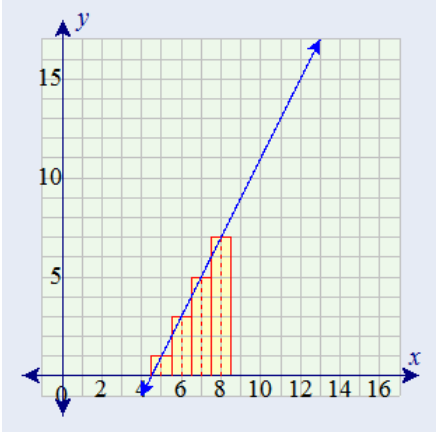
\includegraphics[width=2.60417in]{3_graph.png}
\caption{}
\end{figure}

\subsection{3. Solution}\label{solution-2}

The equation is given as \(2x - 9\), and the ends of the rectangles look
to be 4.5 and 8.5. Since we're looking for the area, we can integrate
this function over these boundaries.

\[
\int_{4.5}^{8.5}(2x - 9)dx
\]

Using the power rule for integration:

\[
(x^2 - 9x)\Big|_{4.5}^{8.5} = \Big[(8.5)^2 - 9(8.5)\Big] - \Big[(4.5)^2 - 9(4.5)\Big]
\\
= [72.25 - 76.5] - [20.25 - 40.5] = 16
\]

\section{4.}\label{section-3}

Find the area of the region bounded by the graphs of the given equations

\[
y = x^2 -2x -2, \ \ \ y = x + 2
\]

\subsection{4. Solution}\label{solution-3}

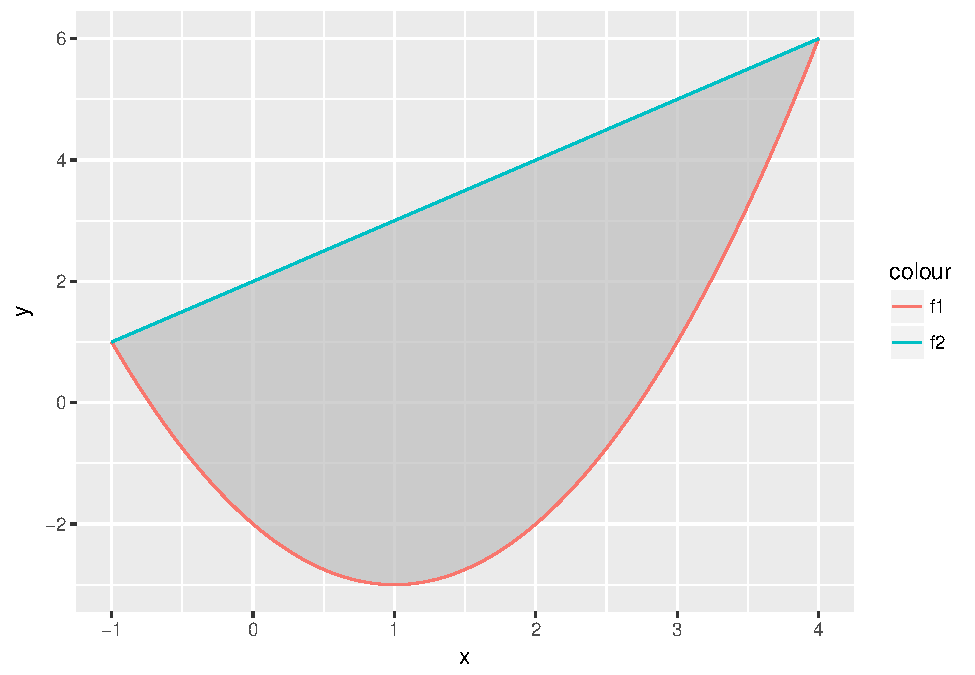
\includegraphics{JSturm_Assignment_13_files/figure-latex/fourgraph-1.pdf}

We're looking for the area between the two functions. The intersection
points are (-1, 1) and (4, 6), which will serve as the boundaries.

\[
A = \int_{-1}^{4} x + 2 \ dx  \ - \ \int_{-1}^{4}x^2 - 2x - 2 dx \\
A = \Big[\frac{1}{2}x^2 + 2x\Big]_{-1}^{4} - \Big[\frac{1}{3}x^3 - x^2 - 2x\Big]_{-1}^{4} \\
= -\frac{1}{3}x^3 + \frac{3}{2}x^2 + 4x\Big|_{-1}^{4} \\
\]

\(\approx\) 20.8333333

\section{5.}\label{section-4}

A beauty supply store expects to sell 110 flat irons during the next
year. It costs \$3.75 to store one flat iron for one year. There is a
fixed cost of \$8.25 for each order. Find the lot size and the number of
orders per year that will minimize inventory costs.

\subsection{5. Solution}\label{solution-4}

I was unsure how to solve this problem, so I googled how to optimize
inventory, and stumbled upon
\href{https://en.wikipedia.org/wiki/Economic_order_quantity}{economic
order quantity (EOQ).}

Quoting the article:

\begin{itemize}
\tightlist
\item
  \(P\) = purchase unit price, unit production cost
\item
  \(Q\) = order quantity.
\item
  \(Q^*\) = optimal order quantity.
\item
  \(D\) = annual demand quantity.
\item
  \(K\) = fixed cost per order, setup cost (not per unit, typically cost
  of ordering and shipping and handling. This is not the cost of goods)
\item
  \(h\) = annual holding cost per unit, also known as carrying cost or
  storage cost (capital cost, warehouse space, refrigeration, insurance,
  etc. usually not related to the unit production cost)
\end{itemize}

The single-item EOQ formula finds the minimum point of the following
cost function:

Total Cost = purchase cost or production cost + ordering cost + holding
cost

Where:

\begin{itemize}
\tightlist
\item
  Purchase cost: This is the variable cost of goods: purchase unit price
  × annual demand quantity. This is P × D
\item
  Ordering cost: This is the cost of placing orders: each order has a
  fixed cost K, and we need to order D/Q times per year. This is K × D/Q
\item
  Holding cost: the average quantity in stock (between fully replenished
  and empty) is Q/2, so this cost is h × Q/2
\end{itemize}

\(TC = PD + \frac{DK}{Q} + \frac{hQ}{2}\).

\(\frac{\text{d}}{\text{d}Q} = -\frac{DK}{Q^2} + \frac{h}{2}\).

We next set this equal to zero, and solve for \(Q\) in order to find the
function minimum.

\(-\frac{DK}{Q^2} + \frac{h}{2} = 0\).

\(Q^{*2} = \frac{2DK}{h} \ \to \ Q^* = \sqrt{\frac{2DK}{h}}\)

We are given these variables, so we just need to plug them into the
formula.

\(D = 110\).

\(K = 8.25\).

\(h = 3.75\).

\[
Q^* = \sqrt{\frac{2\cdot 110\cdot 8.25}{3.75}} = \sqrt{\frac{1815}{3.75}} = \sqrt{484} = 22.
\]

We found 22 to be the lot size per order.

We are given that the store expects to sell \(n = 110\) flat irons. If
there are \(x\) number of irons in each order, our equation is
\(22\cdot x = 110 \ \to \ x = \frac{110}{22} = 5\).

So to minimize inventory costs, the store should make 5 orders of 22
irons per year.

\section{6.}\label{section-5}

Use integration by parts to solve the integral below: \[
\int \ln(9x)\cdot x^6 \ dx
\]

\subsection{6. Solution}\label{solution-5}

The formula for integration by parts is: \[
\int u \ dv = uv - \int v \ du
\]

Let \(u = \ln(9x)\). Using the chain rule
\(du = \frac{1}{9x} \cdot 9 \ dx = \frac{1}{x} \ dx\).

Let \(dv = x^6\), then \(v = \int x^6 = \frac{x^7}{7}\).

Plugging this into the formula:

\[
\ln(9x)\cdot \frac{x^7}{7} - \int \frac{x^7}{7}\cdot \frac{1}{x} \ dx
\]

We can pull out the constant:

\[
\ln(9x)\cdot \frac{x^7}{7} - \frac{1}{7} \int \frac{x^7}{x} \ dx = \ln(9x)\cdot \frac{x^7}{7} - \frac{1}{7} \int x^6 \ dx
\]

Using the power rule for integration:

\[
\ln(9x)\cdot \frac{x^7}{7} - \frac{1}{7} \Big(\frac{x^7}{7}\Big) + C
\]

\[
= \ln(9x)\cdot \frac{x^7}{7} - \frac{x^7}{49} + C
\]

\section{7.}\label{section-6}

Determine whether \(f(x)\) is a probability density function on the
interval \([1, e^6]\). If not, determine the value of the definite
integral.

\[
f(x) = \frac{1}{6x}
\]

\subsection{7. Solution}\label{solution-6}

There are two conditions for a probability density function:

\begin{itemize}
\tightlist
\item
  \(f(x) \geq 0 \ \ \ \forall x\)
\item
  \(\int_{-\infty}^{\infty}f(x) \ dx = 1\)
\end{itemize}

\[
\int_{1}^{e^6} \frac{1}{6x} \ dx = \frac{1}{6} \int_{1}^{e^6}\frac{1}{x} \ dx \\
= \frac{1}{6}[\ln(x)]_{1}^{e^6} \\
= \frac{\ln(e^6) - \ln(1)}{6} = \frac{6\cdot \ln(e) - 0}{6} = \frac{6}{6} = 1
\]

Since the area sums up to 1, we conclude that \(f(x)\) is a pdf on the
interval \([1, e^6]\).


\end{document}
